A pilot study was conducted to verify the method and technical artifact. The benchmarking suite was executed on a 27" Apple iMac Late 2015 running Chrome. The specifications for the iMac, including software versions, are listed in Table \ref{specifications}. Two use cases implemented in C++ was benchmarked using \texttt{performance.now()}\footnote{\url{https://www.w3.org/webperf/}}. The source code for the two use cases is included as Listing \ref{membrane.cpp} at the end of the chapter.

\begin{table}[!h]
\caption{\label{specifications}Specifications of the pilot study desktop computer host.}
\centering
\begin{tabular}{ll}
\hline
\textbf{Model} & Apple iMac 17,1 Late 2015\\ \hline
\textbf{Processor} & Intel Core i5 6500 Skylake 3.2-3.6 GHz, 6 MB shared L3 cache \\
\textbf{Memory} & Corsair Vengeance 2x16 GB 1866 MHz DDR3L SO-DIMM SDRAM \\
\textbf{Storage} & 256 GB SSD \\
\textbf{Graphics} & AMD Radeon R9 M390, 2 GB of GDDR5 SDRAM 30-bit Color \\ \hline
\textbf{Operating System} & Apple macOS 10.14.4 (18E226) \\
\textbf{Web Browser} & Google Chrome 73.0.3683.103 (Official Build) (64-bit) \\ \hline
\end{tabular}
\end{table}

The first use case arithmetic \texttt{add} adds two integers and returns the result. The use case was executed 120 times where the average execution time was $\overline{x}=0.006291666311$ ($s=0.006626145893$) milliseconds when executing the asm.js version and $\overline{x}=0.01045833415$ ($s=0.0095044407$) milliseconds when executing the WebAssembly version. WebAssembly takes longer on average and has a higher standard deviation. The average and standard deviation for the sample is shown in Figure \ref{arithmetic-add-10000-1}a. Figure \ref{arithmetic-add-10000-1}b shows a line graph of all executions. No inferential statistical test was performed since on average asm.js is faster than WebAssembly in this use case. The reason that asm.js is faster than WebAssembly in this particular use case is believed to be because executing using the WebAssembly module is slower than the very low execution for an arithmetic add.

\begin{figure}[!h]%
\centering
\subfloat[]{{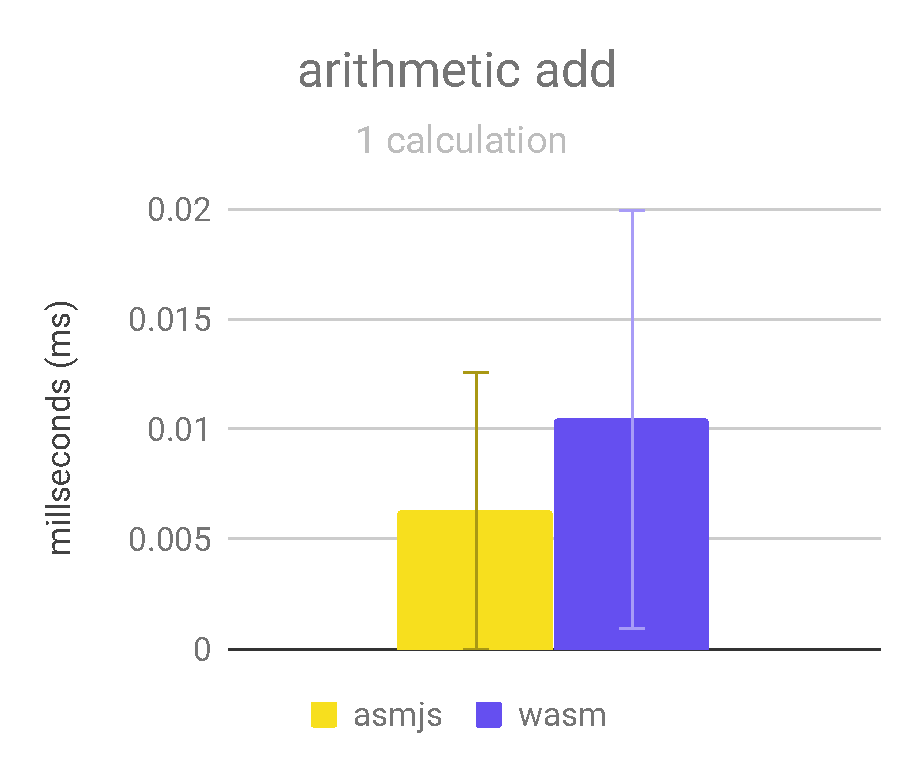
\includegraphics[width=6cm]{../Figures/arithmetic-add-10000-1-column} }}%
%\quad
\subfloat[]{{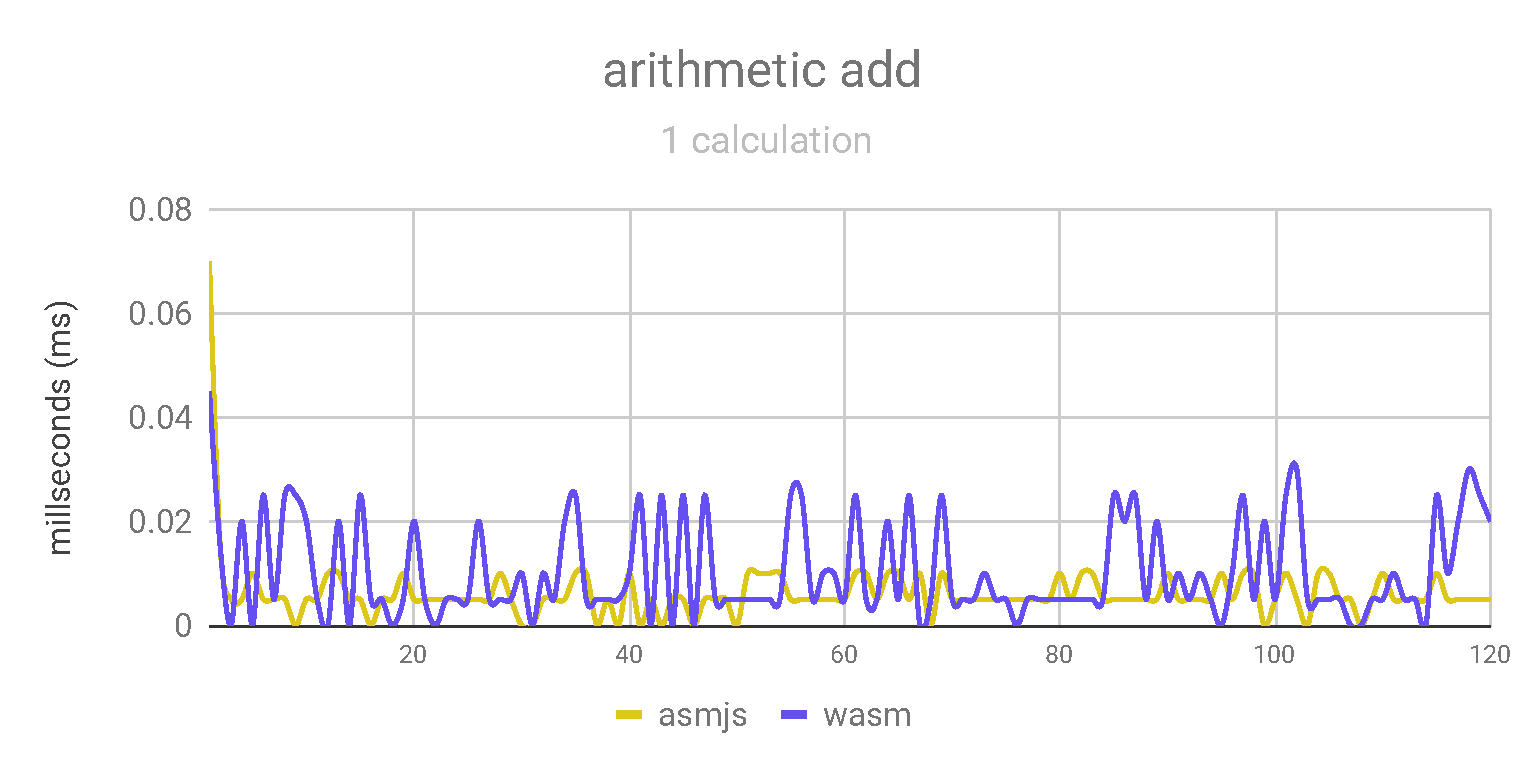
\includegraphics[width=10cm]{../Figures/arithmetic-add-10000-1-line} }}%
\caption{120 executions of a simple arithmetic function that adds two integers.}%
\label{arithmetic-add-10000-1}%
\end{figure}

The values for this use case, produced by Chrome, are very small, much less than a single millisecond. When the same use case was executed in Firefox (not included) those values seemed to be rounded to the nearest millisecond. This behavior is confirmed by the documentation for \texttt{performance.now()} that states that the timestamp produced is not actually high resolution for security reasons\footnote{\url{https://developer.mozilla.org/en-US/docs/Web/API/Performance/now}}. According to the same documentation some browsers might slightly randomize the part of the timestamp that Firefox is rounding. Thus there is a reason to believe that the values shown in Figure \ref{arithmetic-add-10000-1} are slightly randomized by Chrome. The conclusion is that the reliability of the results from benchmarking use cases that take less than a few milliseconds to execute is low, and that such benchmarks should be avoided.

\begin{figure}[!h]%
\centering
\subfloat[]{{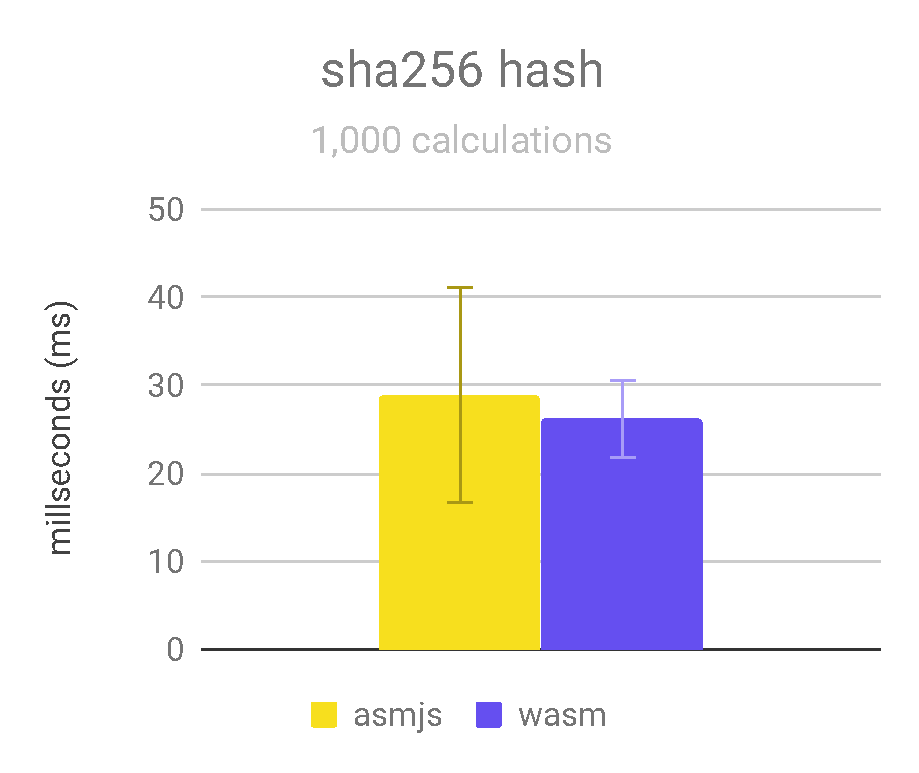
\includegraphics[width=6cm]{../Figures/sha256-hash-1000-1-column} }}%
%\quad
\subfloat[]{{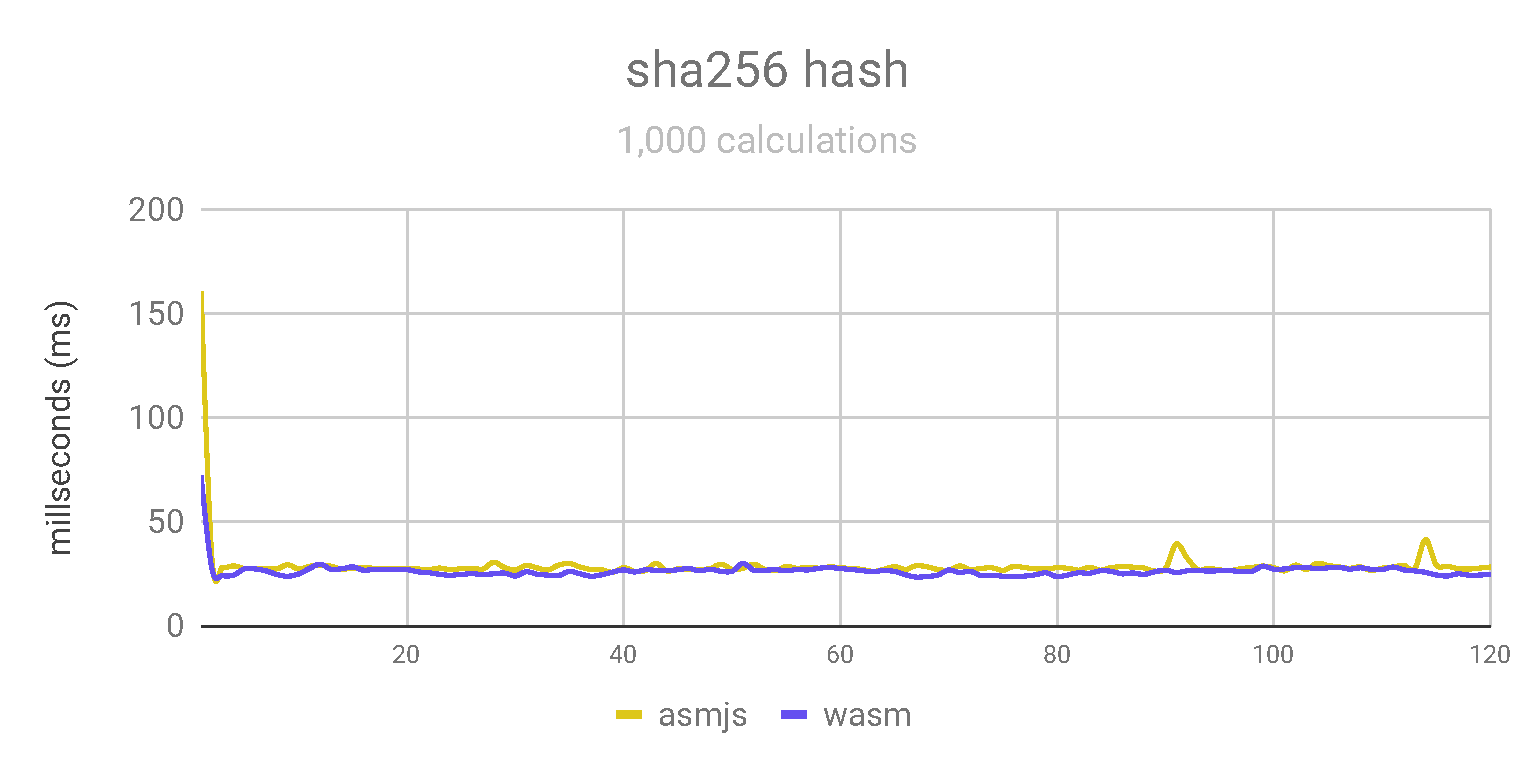
\includegraphics[width=10cm]{../Figures/sha256-hash-1000-1-line} }}%
\caption{120 executions $\times$ 1,000 calculations of a sha256 hash of random strings.}%
\label{sha256-hash-1000-1}%
\end{figure}
    
The second use case calculates a \texttt{sha256} hash for 20 characters long random strings. The sha256 use case was executed 3$\times$120 times. The first round each execution calculated a sha256 hash value for $1,000$ random strings. The average execution time was $\overline{x}=0.006291666311$ ($s=0.006626145893$) milliseconds for the asm.js version and $\overline{x}=0.01045833415$ \\ ($s=0.0.0095044407$) milliseconds for the WebAssembly version. Figure \ref{sha256-hash-1000-1}a shows the average and standard deviation for the sample. Figure \ref{sha256-hash-1000-1}b shows a line graph of all executions. It can be seen in Figure \ref{sha256-hash-1000-1}b that first value is higher than the following values. This is most likely due to the need to bootstrap the Emscripten environment. The same effect can be seen in other line graphs as well, but as the average execution time increases the visibility of the effect decreases. A t-test was calculated on the two independent samples. The result is that $_{0.01}t_{118}=2.299523957$ which is lower than the critical value of $t_{120c}=2.617$ for a one-tailed test with $\alpha = 0.01$. Thus the null hypothesis $H_{0}$ that WebAssembly does \emph{not} have a significantly higher performance than asm.js must be kept. This is not surprisingly as arithmetic add is not an operation with high computational time complexity. The p-value is $0.011171$ so the result would be significant with a alpha higher than $0.011171$, e.g. $\alpha = 0.05$. The result would also be significant if the outlier in the form of the first value was removed and the t-test was performed on only the remaining 119 values. This would give $_{0.01}t_{117}=9.183009699$ which is significantly higher than the same critical value of $t_{120c}=2.617$ for a one-tailed test with $\alpha = 0.01$. 

\begin{figure}[!h]%
\centering
\subfloat[]{{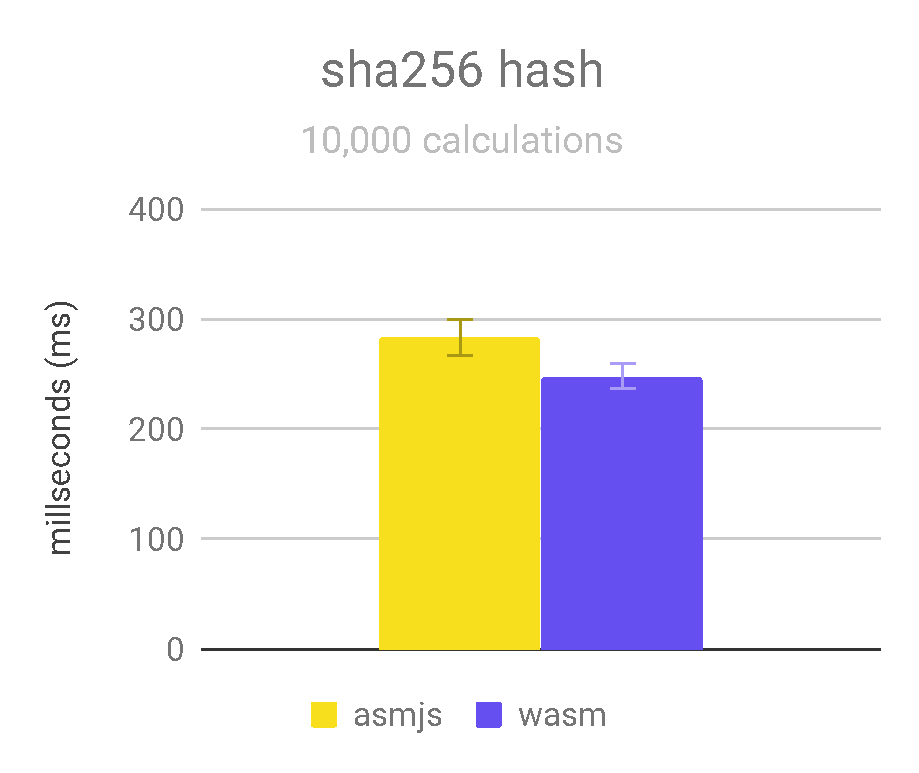
\includegraphics[width=6cm]{../Figures/sha256-hash-10000-1-column} }}%
%\quad
\subfloat[]{{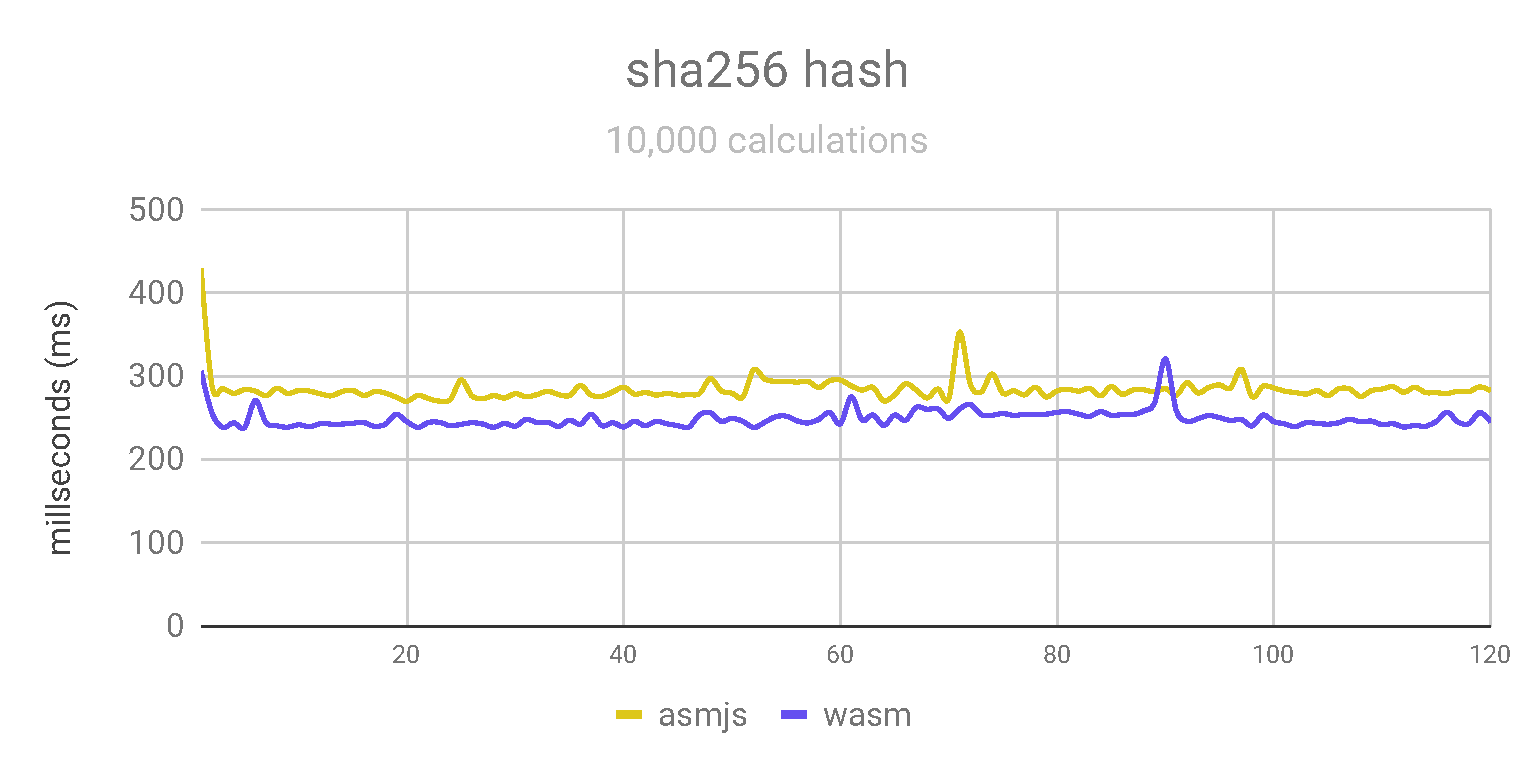
\includegraphics[width=10cm]{../Figures/sha256-hash-10000-1-line} }}%
\caption{120 executions $\times$ 10,000 calculations of a sha256 hash of random created strings.}%
\label{sha256-hash-10000-1}%
\end{figure}
    
The average execution time for $10,000$ random strings was $\overline{x}=283.6995$ ($s=16.36356921$) milliseconds for the asm.js version and $\overline{x}=248.2445417$ ($s=11.27874404$) milliseconds for the WebAssembly version. Figure \ref{sha256-hash-10000-1}a shows the average and standard deviation for the sample and Figure \ref{sha256-hash-10000-1}b shows a line graph of all executions. A t-test shows that $_{0.01}t_{118}=19.54258427$ which is much higher than the critical value of $_{0.01}t_{120c}=2.617$ (one-tailed test with $\alpha = 0.01$). Thus the null hypothesis $H_{0}$ can be rejected in favor of the alternative hypothesis $H_{1}$ that WebAssembly has a significantly higher performance ($\alpha = 0.01$) than asm.js. The p-value is very low ($<0.00001$).

\begin{figure}[!h]%
\centering
\subfloat[]{{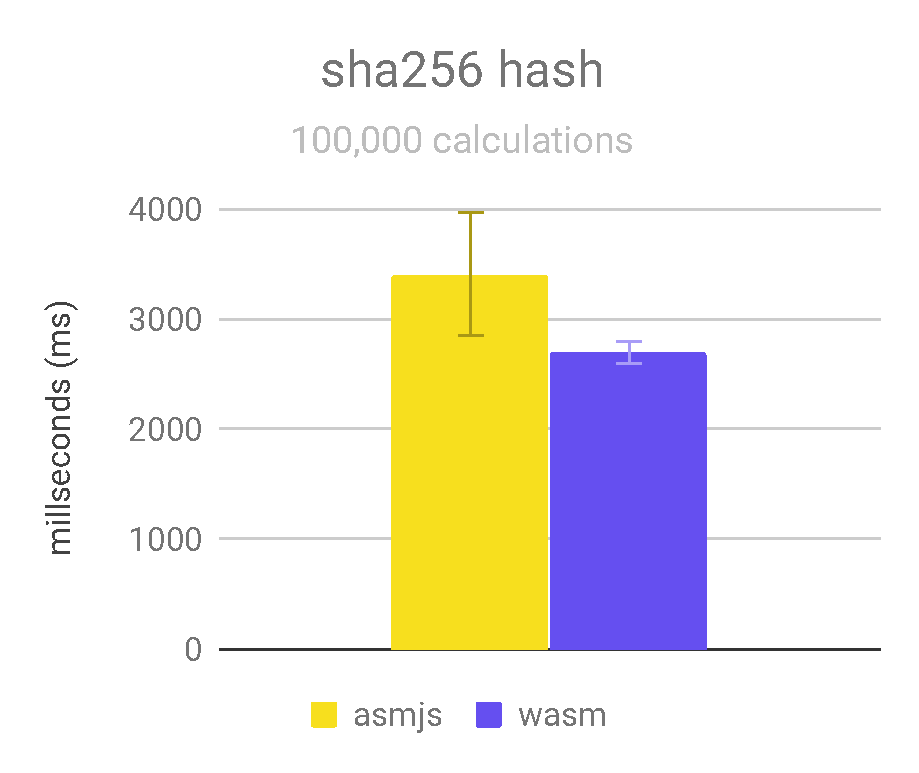
\includegraphics[width=6cm]{../Figures/sha256-hash-100000-1-column} }}%
%\quad
\subfloat[]{{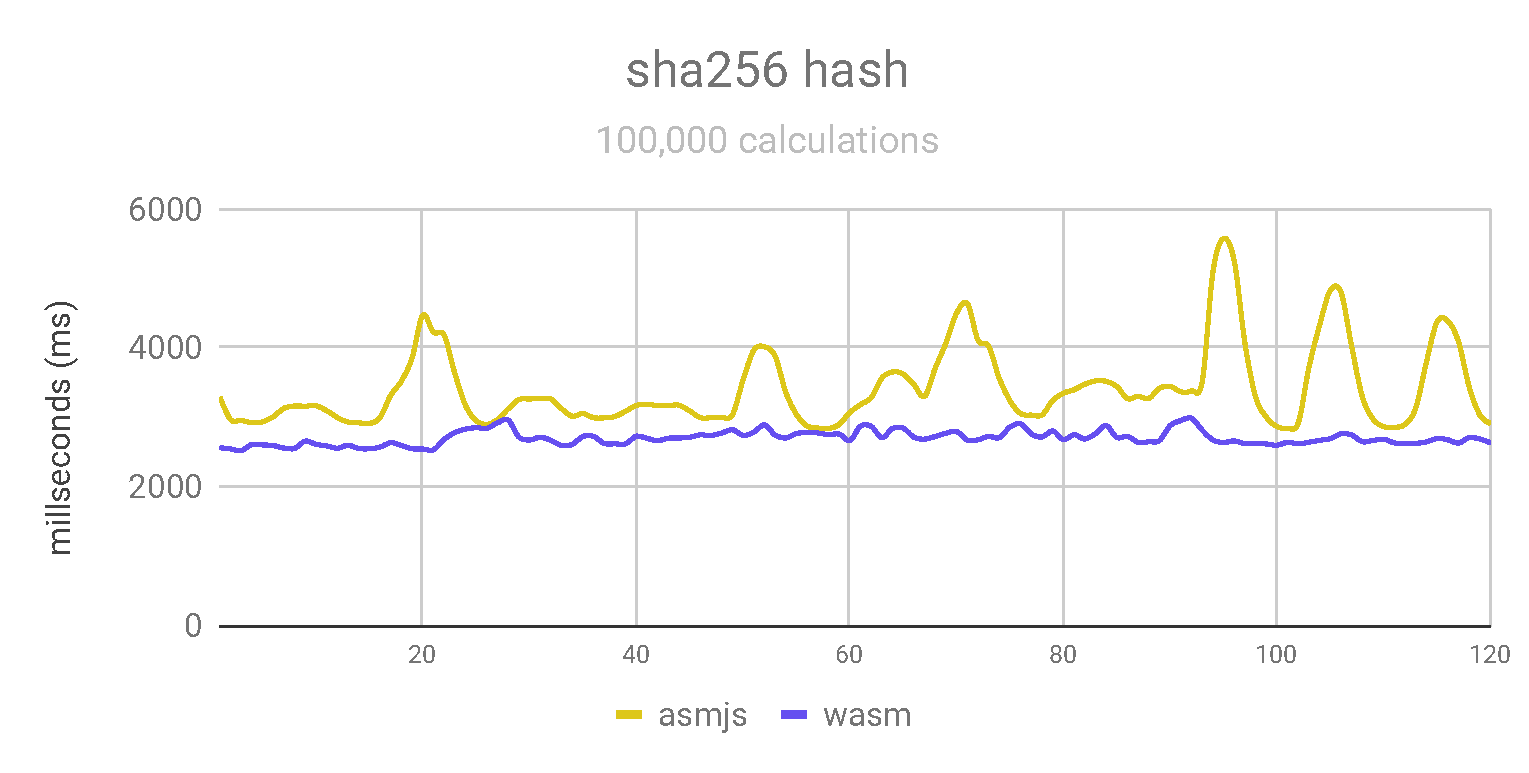
\includegraphics[width=10cm]{../Figures/sha256-hash-100000-1-line} }}%
\caption{120 executions $\times$ 100,000 calculations of a sha256 hash of random created strings.}%
\label{sha256-hash-100000-1}%
\end{figure}

For $100,000$ random strings the average time was $\overline{x}=3409.583083$ ($s=558.0175403$) milliseconds for asm.js and $\overline{x}=2699.307375$ ($s=100.559588$) milliseconds for WebAssembly. Figure \ref{sha256-hash-100000-1}a shows the average and standard deviation for the sample and Figure \ref{sha256-hash-100000-1}b shows a line graph of all executions. WebAssembly not only have a significantly higher performance, the line graphs also show that WebAssembly hash fewer spikes and is thus more predictable which is a stated goal with the WebAssembly compilation target \parencite{HaasRossbergSchuffTitzerHolmanGohmanWagnerZakaiBastien2017}. A t-test gives $_{0.01}t_{118}=13.7223954$ which, although lower than the value for 10,000 calculations, is higher than the critical value $_{0.01s}t_{120c}=2.617$. Thus the null hypothesis $H_{0}$ can be once again be rejected in favor of the alternative hypothesis $H_{1}$. The p-value is lower than $0.00001$.

In the next chapter more use cases will be added and the benchmarking will be executed on in multiple web browsers on a number of computers and mobile devices to know if the result of the pilot study holds true in other scenarios such as part of a mobile web app.

\clearpage

\lstinputlisting[label=membrane.cpp,language=C++,caption=membrane.cpp]{../Listings/membrane.cpp}
